\documentclass[11pt,a4paper]{article}

% --- Encoding & Language ---
\usepackage[utf8]{inputenc}       % Supports UTF-8 input (accents, special chars)
\usepackage[T1]{fontenc}          % Modern font encoding for proper hyphenation
\usepackage[english]{babel}       % Language adaptation (change to your language)

% --- Page Layout & Design ---
\usepackage[margin=1in]{geometry} % Standard 1-inch margins
\usepackage{microtype}            % Improves spacing and justification
\usepackage{parskip}              % Adds space between paragraphs instead of indents
\usepackage{fancyhdr}             % For custom headers and footers
\usepackage{graphicx}             % For including images/logos

% --- Hyperlinks & Color ---
\usepackage[dvipsnames]{xcolor}   % Advanced color support
\usepackage{hyperref}             % Interactive PDF links and URLs
\hypersetup{
    colorlinks=true,
    linkcolor=MidnightBlue,
    filecolor=magenta,
    urlcolor=Cyan,
    citecolor=PineGreen,
    pdftitle={Documentation Title},
    pdfpagemode=FullScreen,
}

% --- Bibliography & Indexing ---
% Using biblatex (modern replacement for traditional bibtex)
\usepackage[backend=biber,style=numeric,sorting=nty]{biblatex}
\addbibresource{references.bib}   % Points to your bibliography file

\usepackage{makeidx}              % For creating an index at the end
\makeindex                        % Initializes the index generator

% -- Plugins for code listings (optional) ---
\usepackage{listings}
\usepackage{xcolor}

% Define custom colors for code highlighting
\definecolor{codegreen}{rgb}{0,0.6,0}
\definecolor{codegray}{rgb}{0.5,0.5,0.5}
\definecolor{codepurple}{rgb}{0.58,0,0.82}
\definecolor{backcolour}{rgb}{0.95,0.95,0.92}

% Configure the look of your code blocks
\lstset{
    backgroundcolor=\color{backcolour},
    commentstyle=\color{codegreen},
    keywordstyle=\color{magenta},
    numberstyle=\tiny\color{codegray},
    stringstyle=\color{codepurple},
    basicstyle=\ttfamily\small,          % Uses monospace font
    breakatwhitespace=false,
    breaklines=true,                     % Wrap long lines automatically
    captionpos=b,                        % Caption at the bottom
    keepspaces=true,
    numbers=left,                        % Line numbers on the left
    numbersep=5pt,
    showspaces=false,
    showstringspaces=false,
    showtabs=false,
    tabsize=4
}

% --- Header/Footer Setup ---
\pagestyle{fancy}
\fancyhf{}
\fancyhead[L]{\small\leftmark}
\fancyhead[R]{\small\thepage}
\renewcommand{\headrulewidth}{0.4pt}

% ==============================================================================
% DOCUMENT METADATA
% ==============================================================================
\title{
    \vspace{2cm}
    \Huge\bfseries Technical Documentation \\
    \large\color{gray}Small Graphics Engine
}
\author{
    \textbf{Ivan Džanija} \\
    \texttt{ivan.dzanija@fer.unizg.hr} \\
    University of Zagreb, Faculty of Electrical Engineering and Computing
}
\date{\today} % Automatically generates today's date, or hardcode it like {June 2026}

% ==============================================================================
% MAIN DOCUMENT
% ==============================================================================
\begin{document}

% --- 1. FRONT PAGE ---
\begin{titlepage}
    \clearpage\thispagestyle{empty}
    \maketitle
    \vfill
    \begin{center}
        % \includegraphics[width=0.3\textwidth]{logo.png}
        \small Version 1.0
    \end{center}
\end{titlepage}

% --- 2. TABLE OF CONTENTS ---
\newpage
\tableofcontents
\newpage

% --- 3. SECTIONS & CONTENT ---
\section{Introduction}
This is the technical documentation for the Small Graphics Engine
project developed for the laboratory exercise in the
Interactive Computer Graphics course at the University of Zagreb.
The purpose of this document is to provide
an overview of the system architecture, design decisions,
and implementation details.


\section{Drawing lines on the screen}
This section describes the algorithm used for drawing lines
on the raster display. The default algorithm
for doing such a task is Bresenham's line algorithm. That is also
the algorithm implemented here, although only for education purposes,
later on the line drawing is done using OpenGL's built-in line
drawing capabilities that fully utilize the GPU's capabilities
for rasterization.
Bresenham's line algorithm here is implemented fully on the CPU, with
manual fragment shading. The screen raster is kept in memory as a 2D
array of pixels.
Here is the code snippet for the manual shading:
\begin{lstlisting}[language=C++, caption=Manual fragment shading example]
// Raster is kept as

// Shades a fragment at the given (x, y) coordinates with the specified color.
int32 Graphics::shade_fragment(int32 x, int32 y, glm::vec3 color) {
  y = _height - 1 - y;  // Invert y-axis
  if (x >= 0 && x < _width && y >= 0 && y < _height) {
    _raster(x, y) = color;
    // _raster[(y * _width * 3) + (x * 3)] = color.x;
    // _raster[(y * _width * 3) + (x * 3) + 1] = color.y;
    // _raster[(y * _width * 3) + (x * 3) + 2] = color.z;
    return 0;
  }
  std::cerr << "ERROR: fragment out of bounds: (" << x << ", " << y << ")" << std::endl;
  return -1;
}
\end{lstlisting}
While the internal representation of the raster is defined as:
\begin{lstlisting}[language=C++, caption=Raster representation example]
struct Raster {
  int32 width{};
  int32 height{};
  std::vector<glm::vec3> data;
};
\end{lstlisting}
As for the line drawing algorithm itself more information (such as full
derivation) can be found
\href{https://en.wikipedia.org/wiki/Bresenham%27s_line_algorithm}{here}.
The snippet of the line drawing algorithm is as follows:
\begin{lstlisting}[language=C++, caption=Bresenham's line algorithm example]
// 0 to 90 degrees
void bresenham_line_1(eng::Graphics &screen, int32 x0, int32 y0, int32 x1, int32 y1,
                      const glm::vec3 &color) {
  const int32 dy = y1 - y0;
  const int32 dx = x1 - x0;
  if (dy <= dx) {
    const int32 change = dy << 1;       // 2 * dy
    const int32 correction = -dx << 1;  // -2 * dx

    int32 y_curr = y0;
    int32 y_cal = -dx;
    for (int32 x_curr = x0; x_curr <= x1; ++x_curr) {
      screen.shade_fragment(x_curr, y_curr, color);
      y_cal += change;
      if (y_cal >= 0) {
        ++y_curr;
        y_cal += correction;
      }
    }
  } else {
    const int32 change = dx << 1;       // 2 * dx
    const int32 correction = -dy << 1;  // -2 * dx

    int32 x_curr = x0;
    int32 x_cal = -dy;
    for (int32 y_curr = y0; y_curr <= y1; ++y_curr) {
      screen.shade_fragment(x_curr, y_curr, color);
      x_cal += change;
      if (x_cal >= 0) {
        ++x_curr;
        x_cal += correction;
      }
    }
  }
}
\end{lstlisting}



\section{Drawing and shading polygons}
In this section we describe the algorithm for drawing
and shading polygons. To be more precise we are talking about
convex polygons, as the algorithm for concave polygons is more
complex and is not implemented here.
In this section we are still doing the drawing and shading on the CPU,
with manual fragment shading as this is this educational implementation
and most of the Graphics API's (such as OpenGL) provide built-in
functionality for drawing and shading polygons
that fully utilize the GPU's capabilities.
First thing we are doing is providing a user with a way to define
a polygon. When the user presses the left mouse button the application
records the position of the mouse cursor and adds it to the list of
polygon vertices. If the vertex just added would form a non-convex
polygon the user is alerted in the console. The checking is done
by seeing if all the vertices of the polygon are on the same side
of the line formed by any two vertices of the polygon. If that is not
the case then the polygon is not convex.
Here is the code snippet for checking if a polygon is convex:
\begin{lstlisting}[language=C++, caption=Convex polygon checking example]
[[nodiscard]] std::optional<bool> test_convex() const {
  if (_elements.size() < 3) {
    return std::nullopt;  // Not enough vertices to determine convexity
  }
  uint8 negative = 0;
  uint8 positive = 0;
  for (size_t i = 0; i < _elements.size(); ++i) {
    const auto &curr_edge =
        _elements[(i + _elements.size() - 1) % _elements.size()].edge;
    const auto &next_point = _elements[(i + 1) % _elements.size()].point;
    double dot =
        (curr_edge.a * next_point.x) + (curr_edge.b * next_point.y) + curr_edge.c;
    if (dot < 0) {
      ++negative;
    }
    if (dot > 0) {
      ++positive;
    }
  }
  return (negative == 0 || positive == 0);
}
\end{lstlisting}
The the user finishes defining the polygon by pressing the right mouse
button the last line between the last vertex and the first vertex
is drawn. After that the polygon is filled using the scanline
algorithm. The scanline algorithm works by iterating through
each scanline (horizontal line) of the raster
and finding the intersection points between the scanline and the
left and right edges of the polygon. Specifically for each scanline
we are looking for the leftmost right edge and the rightmost left edge.
After that we are filling the pixels between those two edges using the
Bresenham's line algorithm described in the previous section.
The code snippet for the scanline algorithm is as follows:
\begin{lstlisting}[language=C++, caption=Scanline algorithm example]
void draw_filled(eng::Graphics &screen) {
  if (_elements.empty()) {
    // std::cerr << "Polygon has no vertices to draw." << std::endl;
    return;  // No vertices to draw
  }

  int32 x_min = _elements[0].point.x;
  int32 x_max = _elements[0].point.x;
  int32 y_min = _elements[0].point.y;
  int32 y_max = _elements[0].point.y;
  double L;
  double R;

  for (const auto &element : _elements) {
    x_min = std::min(x_min, element.point.x);
    x_max = std::max(x_max, element.point.x);
    y_min = std::min(y_min, element.point.y);
    y_max = std::max(y_max, element.point.y);
  }

  for (int32 y = y_min; y <= y_max; ++y) {
    L = static_cast<double>(x_max);
    R = static_cast<double>(x_min);
    for (const auto &curr : _elements) {
      if (curr.edge.a == 0) {
        continue;  // Skip horizontal edges
      }
      double x = (-curr.edge.b * y - curr.edge.c) / static_cast<double>(curr.edge.a);
      if (test_orientation() == PolyOrientation::CLOCKWISE) {
        if (curr.left) {
          L = std::min(L, x);
        } else {
          R = std::max(R, x);
        }
      } else {
        if (curr.left) {
          R = std::max(R, x);
        } else {
          L = std::min(L, x);
        }
      }
    }
    eng::draw_line(screen, static_cast<int32>(L + 0.5F), y,
                   static_cast<int32>(std::round(R + 0.5F)), y);
  }
  // Draw starting vertex in red and outline in blue for clarity
  screen.shade_fragment(_elements[0].point.x, _elements[0].point.y,
                        glm::vec3(1, 0, 0));
  draw_outline(screen);
}
\end{lstlisting}
The final thing supported by the application is tesing if the point
is inside the polygon. This is done by counting the number
of times a ray from the point intersects the edges of the polygon.
The user defines a point by pressing the left mouse button while in
polygon testing mode. If the number of the intersections is odd then
the point is inside the polygon, otherwise it is outside.
Example are shown in the picture \ref{fig:point_in_polygon}.
\begin{figure}[ht]
    \centering
    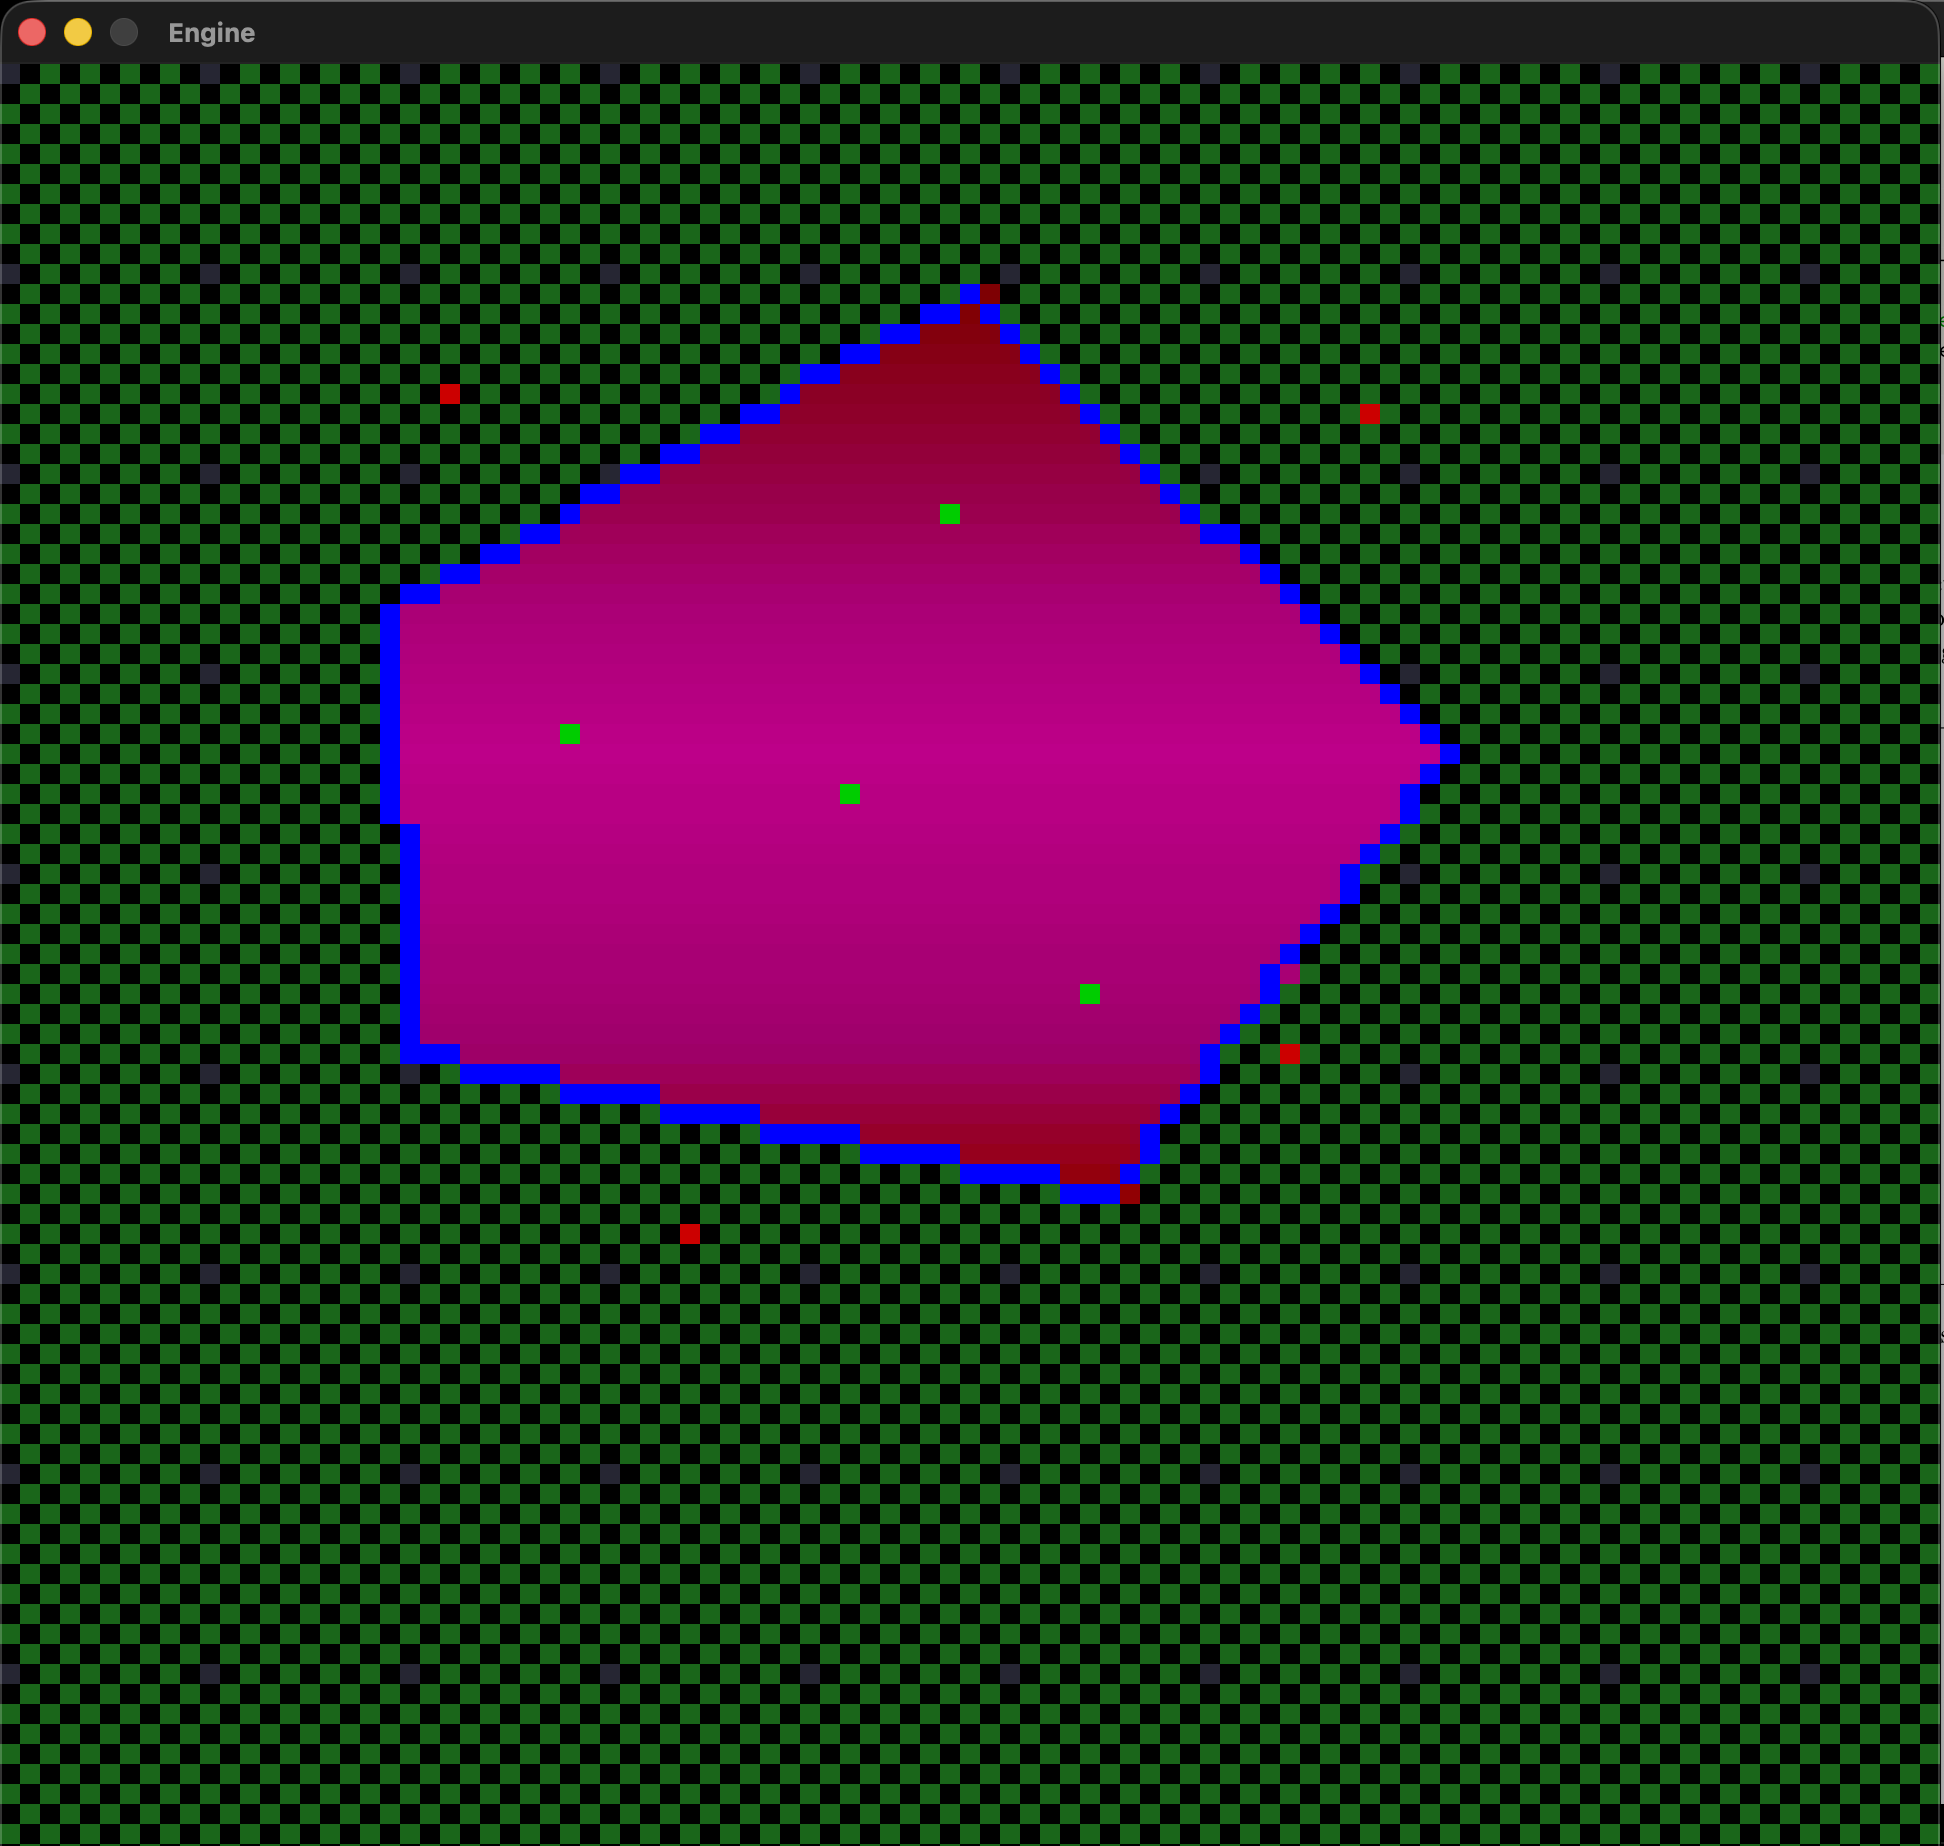
\includegraphics[width=0.5\textwidth]{figures/point_in_polygon.png}
    \caption{Example of point-in-polygon testing.
    The red point is outside the polygon,
    while the green point is inside.}
    \label{fig:point_in_polygon}
\end{figure}


\section{Starting with OpenGl}
Until now we have been doing all the drawing and shading on the CPU,
with manual fragment shading and just forwarding the final
raster to the GPU for displaying. However, this is higly inefficient
and we are now switching to using OpenGL's built-in functionality
to fully utilize the GPU's capabilities for rasterization.
In this part we will be defining and operating with OpenGL's
pipeline.
In the following picture \ref{fig:basic_coloring}
you can see the final result of the current stage of the application.
The top left corner is just the display for the currently selected
color. While the triangles are drawn using OpenGL's built-in triangle
primitives. The triangles are colored using the color defined in the
top left corner and the color is interpolated across the triangle.
All of this is done using OpenGL's built-in functionality
and the GPU's capabilities. Only thing we do here is record the position
of the mouse cursor when the user clicks and update the corresponding
vertex buffer.
\begin{figure}[ht]
    \centering
    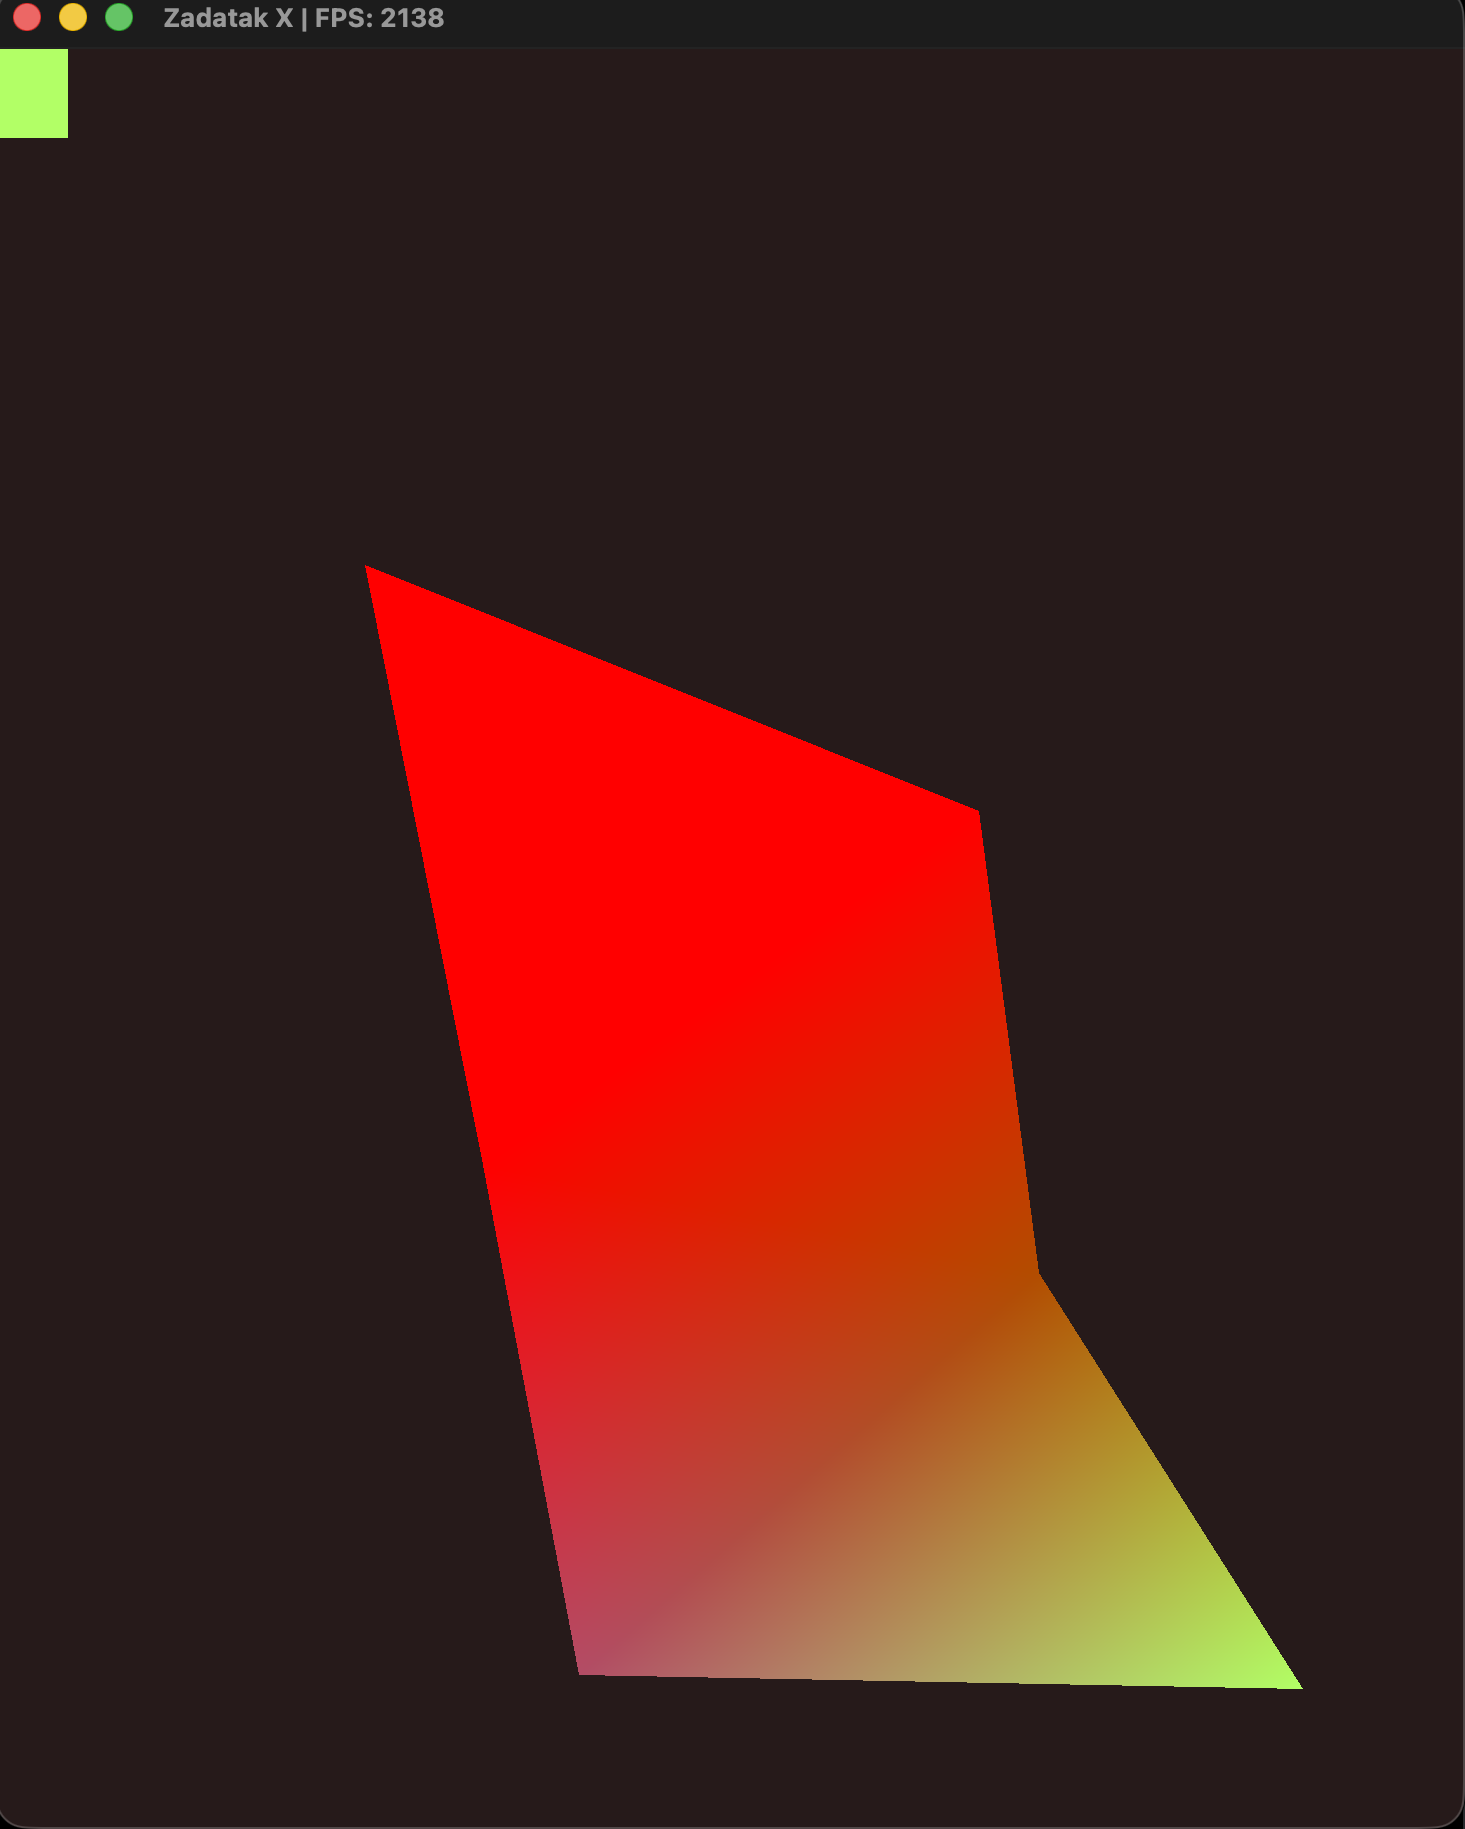
\includegraphics[width=0.5\textwidth]{figures/basic_coloring.png}
    \caption{Example of basic triangle coloring using OpenGL's built-in functionality.}
    \label{fig:basic_coloring}
\end{figure}
\\
OpenGL's features we introduced here are vertex and fragment shaders,
vertex buffer objects (VBOs), vertex array objects (VAOs)
and element buffer objects (EBOs).
Vertex and fragment shaders we used here are the most basic ones
that just pass the vertex positions and colors to the GPU and let
the GPU handle the rasterization and interpolation. The VBOs are used
to store the vertex data (positions and colors) on the GPU,
while the VAOs are used to store the state of the vertex attributes
(such as the layout of the vertex data).
The EBOs are used to store the indices of the vertices when we
going with indexed approach.\\
\section{3D Models}
Following the section where we introduced OpenGL into our application
we now want to jump from 2D space to 3D space and start
working on 3D models. First thing we need to do is define a
good architecture for the rest of the application since we will be
using this as a base for the rest of the development. The beginning
idea for the architecture
is given in the following picture \ref{fig:architecture}.
\begin{figure}[ht]
    \centering
    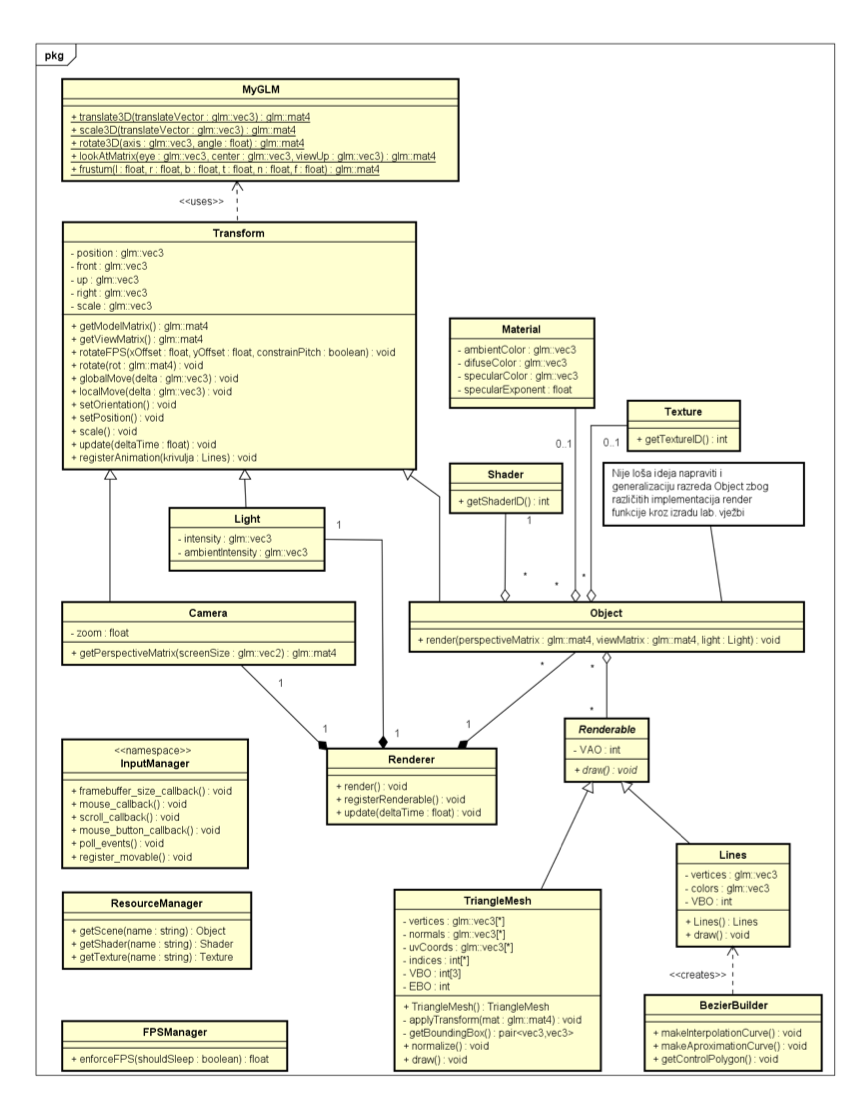
\includegraphics[width=0.8\textwidth]{figures/architecture.png}
    \caption{Architecture of the application.}
    \label{fig:architecture}
\end{figure}
\\
Although some small changes were made later on we will keep this
here since for now this was a plan and the mental model.
After we have the architecture defined we start building the pieces.
First thing we are doing is defining a way to load 3D models
from files. We are using the OBJ file format for storing 3D models
and using external library Assimp for loading the models from files.
All models are represented by the class Renderable that is just
an abstract interface for rendering something on the screen. In this
section we are focusing on loading models and for that we introduce
another class Mesh that is responsible for storing the vertex data
(positions, normals, texture
coordinates) and the indices of the vertices.
The Renderable class has a method draw() that is
responsible for rendering the model on the screen.
Other pieces we introduce here are Object class and Renderer class.
We will start with the Object class and it is responsible for
storing the shader and all the meshes that make up the model.
The Renderer class is responsible for rendering all the objects
on the screen and it keeps track of all the objects in the scene with
methods for adding and removing objects from the scene.
The final things we introduce are the ResourceManager class and
the ObjectLoader class. The ResourceManager is the owner off
all the objects and resources in the application and it caches
everything inside appropriate data structures like
\texttt{std::unordered\_map} for easy access. When some resource is
needed somewhere in the application it is requested from the
ResourceManager. From there there are two options, either
the resource is already cached and we return a \texttt{std::shared\_ptr}
to the resource or the resource is not cached then we use the other
mentioned class ObjectLoader that is just a clean facade pattern
for using the Assimp library for loading the models from files.
After the model is loaded it is first normalized on the screen
and then cached in the ResourceManager. After the model is loaded
and cached then we return a \texttt{std::shared\_ptr} to
the model and it is used in the application.

\section{Math and transformations}
This is probably the hardest part of the application when doing
manually. In this section we introduce the math library GLM,
classes like Transform and TransformGenerator and the concept of
camera. We will start with the Transform class. The idea
of the Transform class is to provide a clean interface for
everything that will be in the scene and needs to track its position,
rotation and scale. The Transform class is abstract class from which
Camera and Object classes inherit. Transform class iternally keeps
track of the position, local axes and scale of the object. It provides
methods for rotating, moving and scaling the object in the scene.
These methods all just internally update the position, local axes
and scale. This movement is then represented as a transformation
matrix that the application fetches with method
\texttt{get\_model\_matrix()} and sends the model matrix to the shader
for rendering.
Another class we introduce is the TransformGenerator class. This
class is just a clean facade pattern for generating transformation
matrices using the GLM library.
The final thing introduced here is the concept of camera encapsulated
in the Camera class. The Camera class inherits from the Transform class
and only thing it is reponsible for is generating the view and
projection matrices. The view matrix is generated using
\texttt{glm::lookAt()} function from the GLM library
and the projection matrix is generated using \texttt{glm::frustum()}
function from the GLM library (rather the abstracted versions inside
the TransformGenerator class).
With all this we finally arrive at the shaders. Fragment shader
has stayed the same and we are not making changes now. The vertex shader
has a small change. Now we are sending the model, view and
projection matrices to the vertex shader and then all the transformations
are done in the vertex shader (meaning on the GPU). The vertex shader
looks as follows:
\begin{lstlisting}[language=C, caption=Vertex shader example]
#version 330 core
// Input
layout (location = 0) in vec3 aPos;
layout (location = 1) in vec3 aCol;

// Matrix
uniform mat4 u_model;
uniform mat4 u_view;
uniform mat4 u_projection;

// Color
uniform vec3 u_color;

// Output
out vec3 color;

void main() {
  color = aCol;
  gl_Position = u_projection * u_view * u_model * vec4(aPos, 1.0);
}
\end{lstlisting}
After all this we finally have a working application that can load
3D models from files, render them and move around the scene.
The preview of the application at this stage is shown in the following
picture \ref{fig:3d_preview}. In the picture we can also see the
local axes of the models and global axes of the scene.
\begin{figure}[ht]
    \centering
    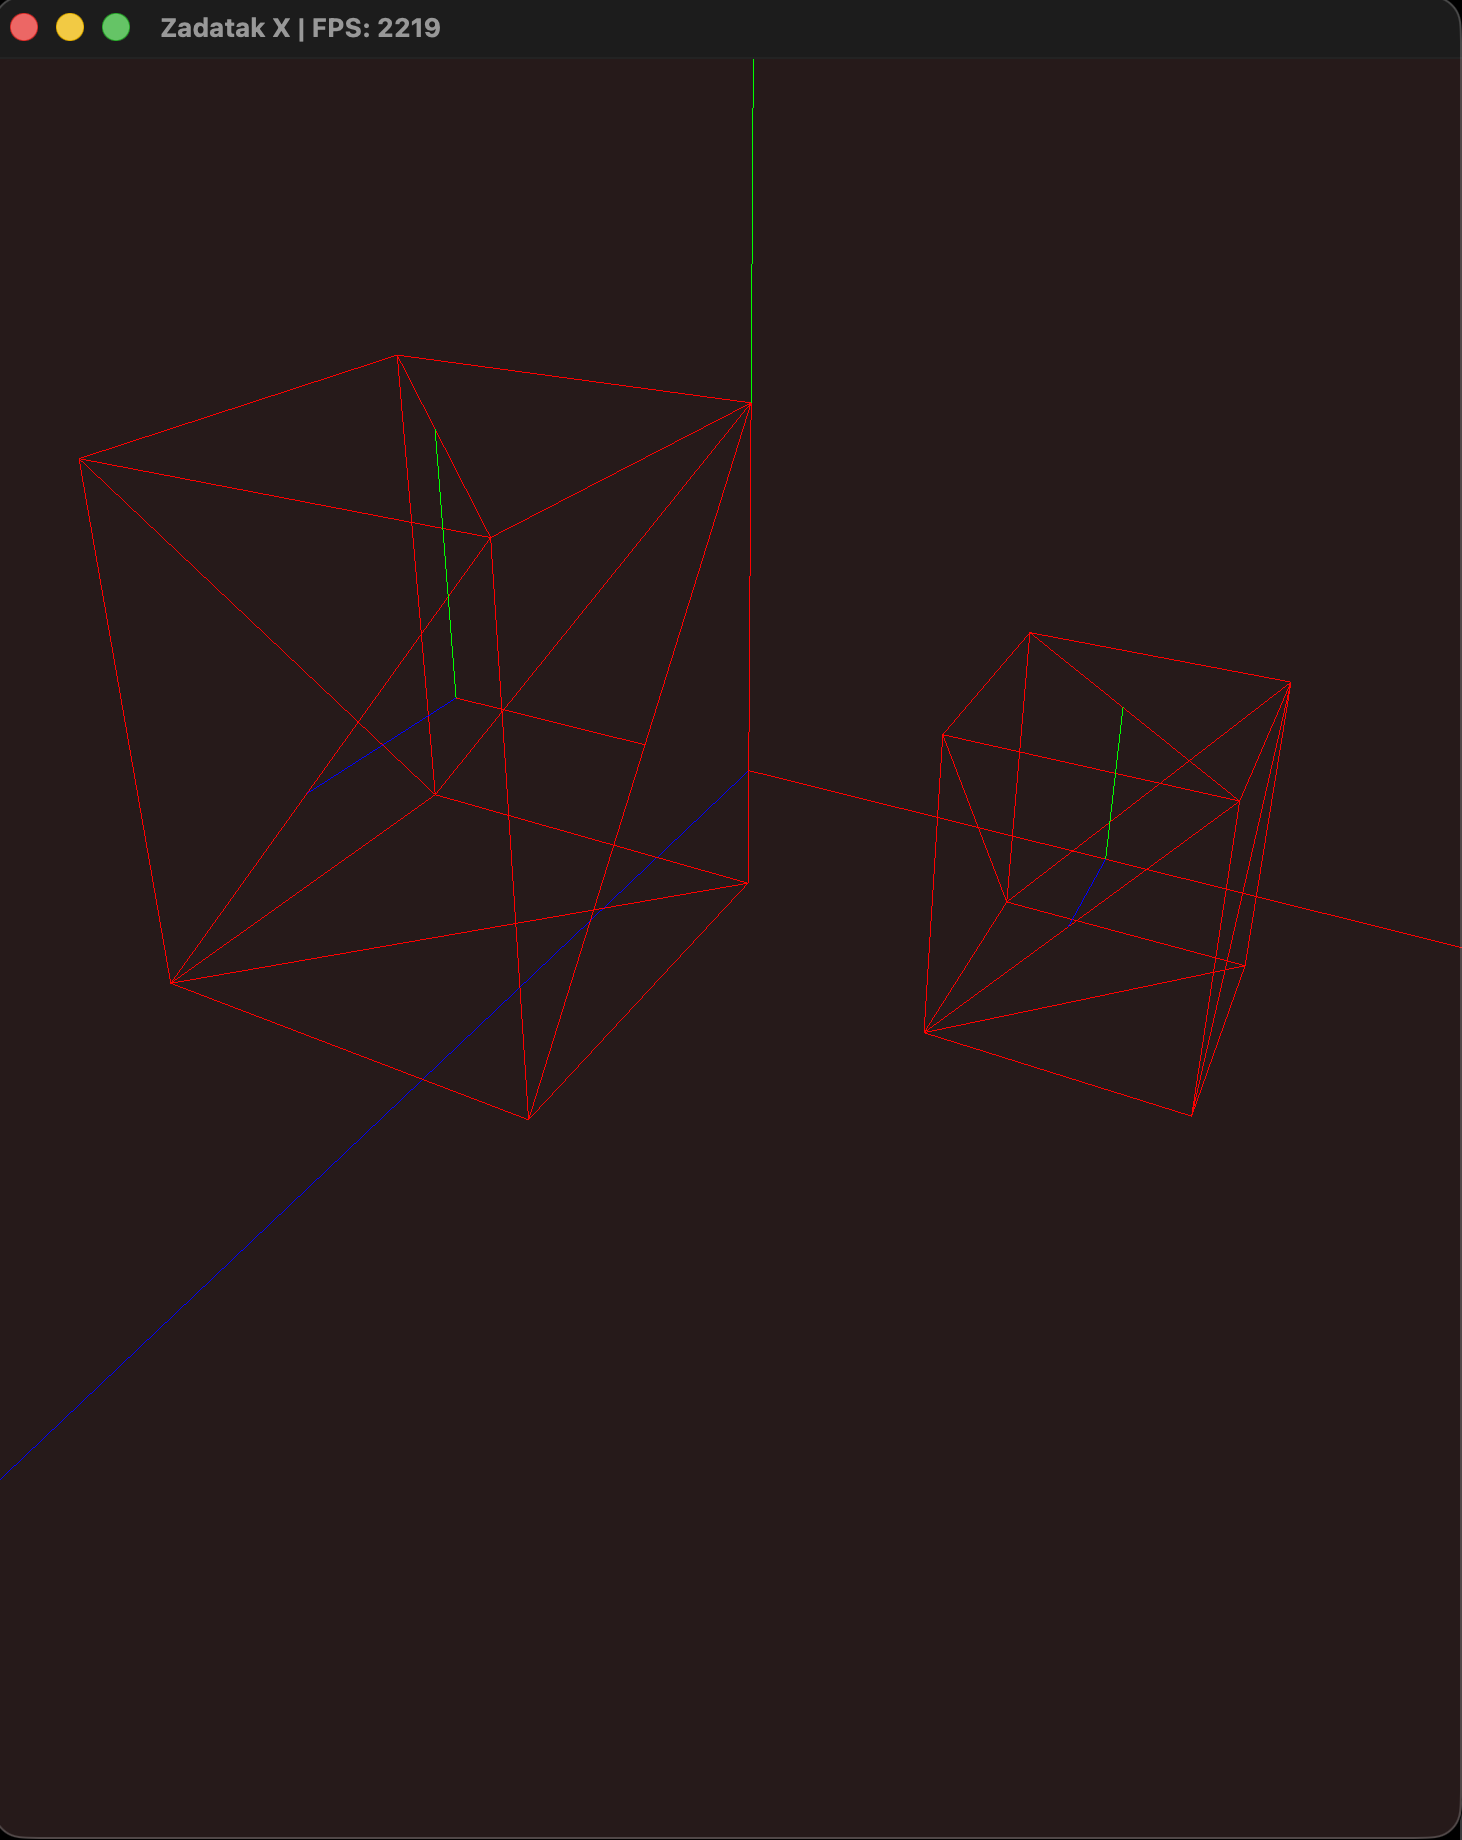
\includegraphics[width=0.5\textwidth]{figures/3d_preview.png}
    \caption{Preview of the application at the stage of 3D model loading and rendering.}
    \label{fig:3d_preview}
\end{figure}

\section{Back-face culling}
This is a small optimization technique that we can implement to improve
the performance of our application. The idea is to not render any
faces of the model that are facing away from the camera. This can be
done a lot of different ways. We have tried two approaches for
educational purposes. Both approaches are done inside the geometry
shader. The first approach is done in the scene coordinate system
where we calculate the \textit{centroid} of the triangle and then
calculate the normal of the triangle. After that we calculate the vector
from the camera to the centroid and then we calculate the dot product
between the normal and the vector from the camera to the centroid.
The dot product gives us the angle between the normal and the vector
from the camera to the centroid. If the angle is greater than 90
degrees then the face is facing away from the
camera and we can discard it. The second approach is done in the view
coordinate system where we just have to check that the order of the
vertices is counter-clockwise (or clockwise depending on the convention)
to determine if the face is facing towards or away from the camera.
This is done by calculating the cross product of the
two edges of the triangle and then checking the sign
of the z component of the cross product.
Both of these approaches give us the same result but in the next
iterations of the application we will be using OpenGL's built-in
back-face culling functionality using the following code snippet:
\begin{lstlisting}[language=C++, caption=OpenGL back-face culling example]
// Enable back-face culling
glEnable(GL_CULL_FACE);
glCullFace(GL_BACK);
\end{lstlisting}
Using OpenGL's built-in functionality is much more efficient since
it is done on the GPU and it is optimized for performance.

\section{Bezier curves}
In this section we introduce the concept of Bezier curves and how to
implement them in our application. Bezier curves we use here
are approximate Bezier curves and interpolation Bezier curves. The
difference is that the approximate Bezier curves do not necessarily
pass through the control points while the interpolation Bezier curves
do pass through the control points. The user defines the control points
by pressing the right mouse button while in Bezier curve mode. After enough
added points the user can switch to the curve drawing mode by
pressing the space bar and then both types of Bezier curves are drawn
on the screen. If the user continues holding the space bar the camera
starts following the interpolation Bezier curve while rotating to follow
the slope of the current point on the curve.
The code snippet for calculating the points
on the Bezier curve is as follows:
\begin{lstlisting}[language=C++, caption=Bezier curve calculation example]
[[nodiscard]] std::vector<CurveVertex> BezierBuilder::build_approximate(
    size_t num_segments) const {
  if (_control_points.empty()) {
    std::cerr << "ERROR: No control points provided for Bezier curve approximation."
              << std::endl;
    return {};
  }

  size_t n = _control_points.size() - 1;
  auto binomial_coefficients = _precalculate_binomial_coefficients(n);
  glm::vec3 color = {1.0F, 0.0F, 1.0F};

  std::vector<CurveVertex> vertices;
  vertices.reserve(num_segments + 1);

  float delta = 1.0F / num_segments;

  for (size_t i = 0; i <= num_segments; ++i) {
    glm::vec3 point(0.0F);
    const float t = i * delta;
    for (size_t j = 0; j <= n; ++j) {
      float coeff = binomial_coefficients[j] * std::pow(t, j) * std::pow(1 - t, n - j);
      point += coeff * _control_points[j];
    }
    vertices.emplace_back(point, color);
  }
  return vertices;
}
\end{lstlisting}
After this the collection of points on the curve is stored inside a new
class Curve that inherits from the Renderable class. It is then registered
into the Renderer and rendered on the screen with the rest of the scene.
An example of the Bezier curve is shown in the following picture \ref{fig:bezier_curve}.
\begin{figure}[ht]
    \centering
    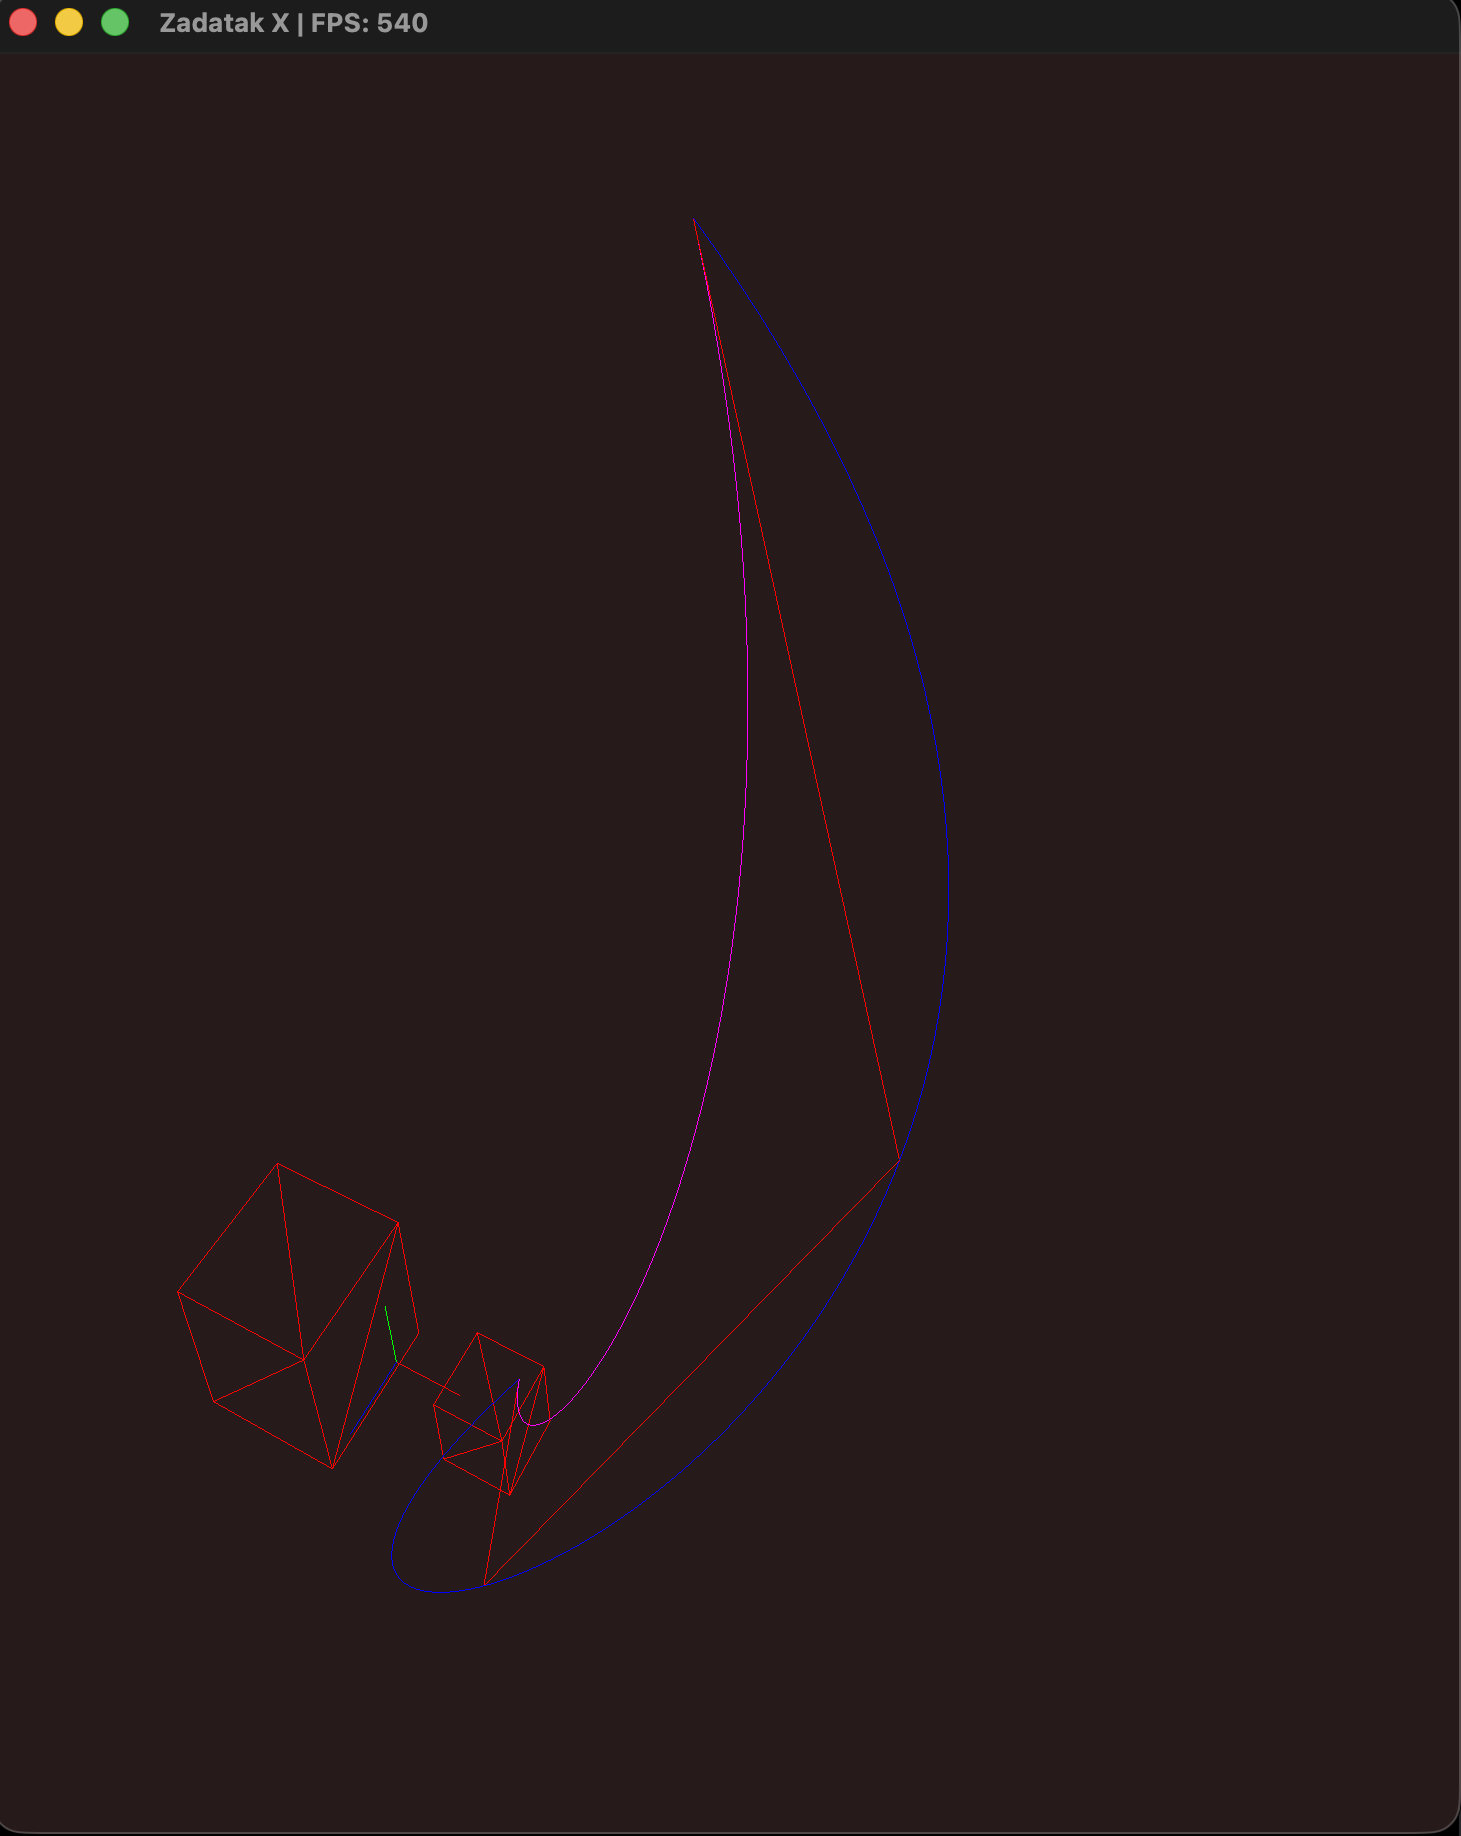
\includegraphics[width=0.5\textwidth]{figures/bezier_curve.png}
    \caption{Example of Bezier curve drawing. The magenta curve is the approximate Bezier curve
    while the blue curve is the interpolation Bezier curve.}
    \label{fig:bezier_curve}
\end{figure}
\section{Lighting, textures and shading}
In this section we introduce the concept of lighting,
textures and shading.
For lighting we educationally implement the constant shading,
Gouraud shading and Phong shading. The constant shading is the simplest
one where we just calculate the color of the face based on the normal
of the face and the light direction and then we use that color for the entire face. The Gouraud shading is a bit more complex where we calculate
the color of the vertices based on the normal of the vertices and the light direction and then we
interpolate the colors across the face. Phong shading is the most complex
where we calculate the color of the fragments based on the normal of the fragments
and the light direction.
In the actual implementation the only difference is between where the shading
is done. In the constant shading we are doing all these calculations inside
the geometry shader and then we just pass the color to the fragment shader.
In the Gouraud shading we are doing all these calculations inside the vertex shader
and then we just pass the color to the fragment shader (since the color
will be interpolated).
In the Phong shading we are passing the normal of the fragment to the fragment shader
and then we are doing all the calculations inside the fragment shader. This
just means that in the Phong shading we are interpolating the normals and
in the Gouraud shading we are interpolating the colors.
Example of the different shading techniques is shown in the following picture \ref{fig:shading}.
In the actual implementation we are using the Phong shading model since it gives us the best visual
results and it is the most realistic one.
The constant shading and Gouraud shading are just implemented for
educational purposes to show the difference between
the different shading techniques.
\begin{figure}[ht]
    \centering
    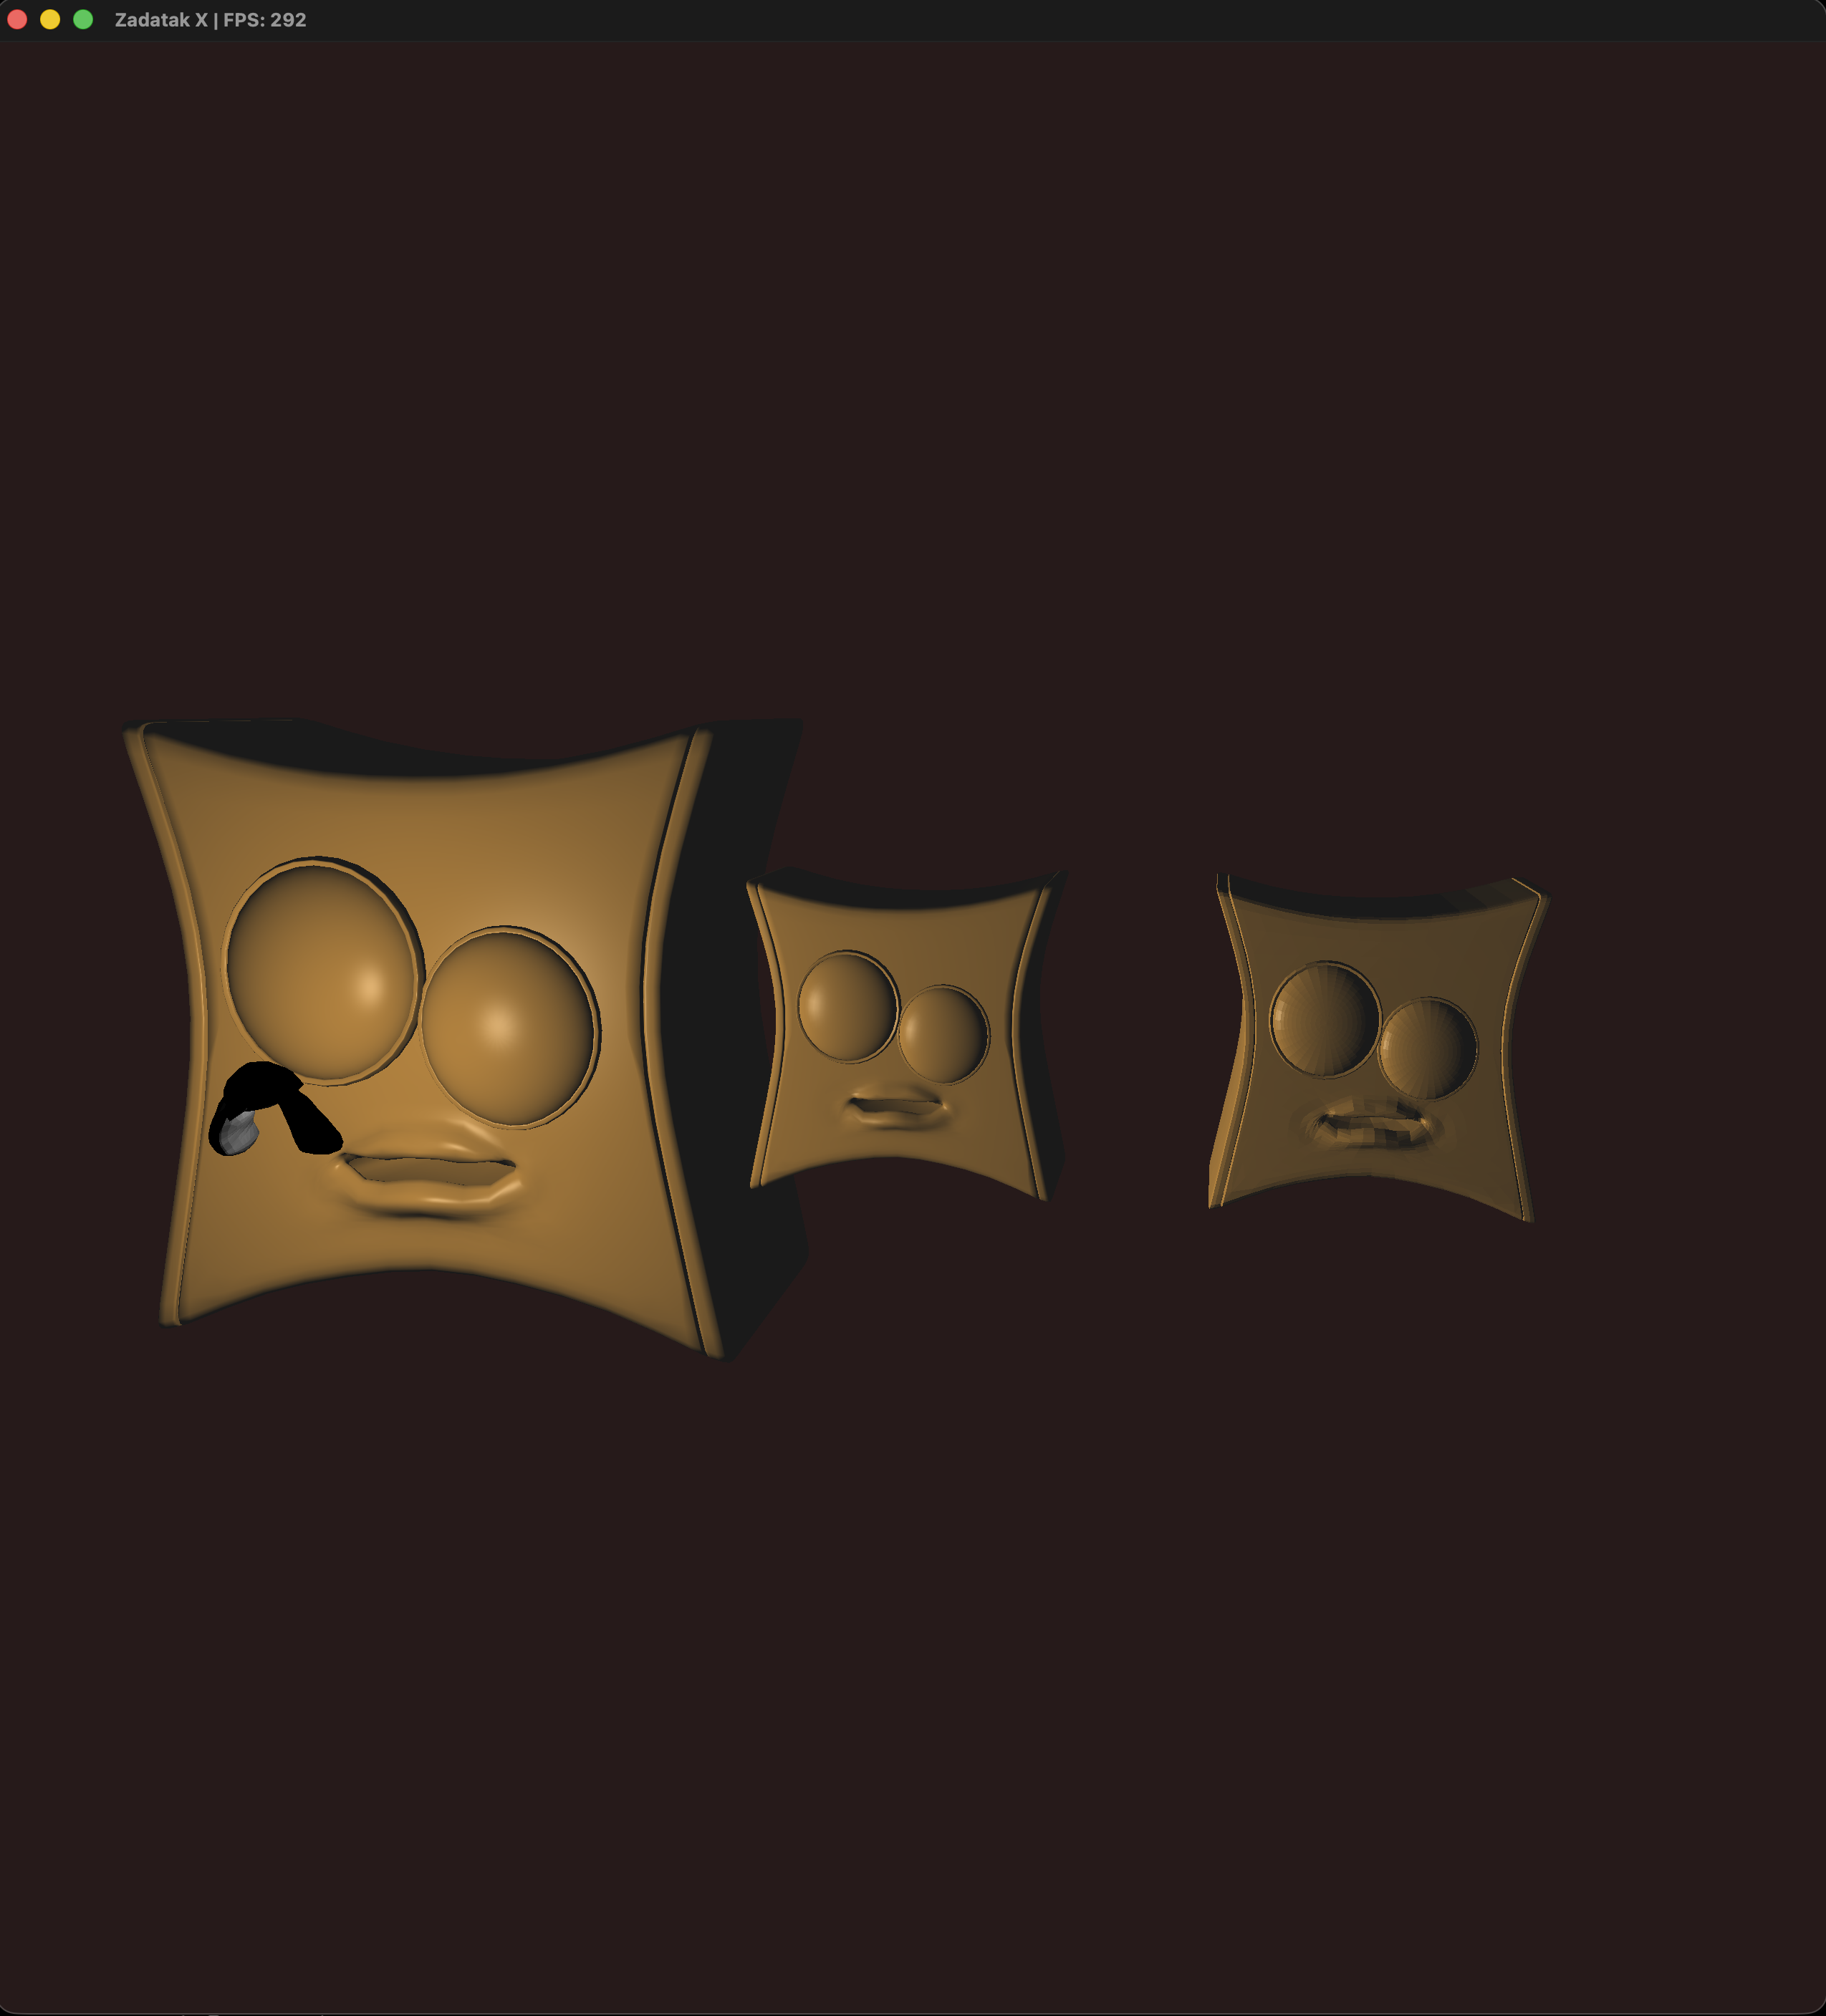
\includegraphics[width=0.5\textwidth]{figures/shading.png}
    \caption{Example of different shading techniques.
    The left head is shaded with Phong shading,
    the middle head is shaded with Gouraud shading and
    the right head is shaded with constant shading.}
    \label{fig:shading}
\end{figure}
\\

Following the basic lighting models, we expanded the engine
by implementing 2D texture mapping.
Textures are loaded from image files using
the \texttt{stb\_image} library inside our resource management
pipeline and sent to the GPU as texture objects.
To support this, the Vertex structure is updated to include
UV coordinates, which are automatically
interpolated across the surface of the polygons.
After this we just update the fragment shader (we are using the
Phong shading model here) to sample the diffuse and specular textures
and incorporate them into the final lighting calculations.
The following code snippet shows the fragment shader
where the texture sampling and lighting calculations are done:
\begin{lstlisting}[language=C, caption=Fragment shader texture sampling snippet]
#version 330 core

in vec3 v_normal;
in vec3 v_world_pos;
in vec2 v_tex_coords;

struct Light {
  vec3 position;
  vec3 intensity;
  vec3 ambient;
};
uniform Light u_light;

struct Material {
  sampler2D diffuse1;
  sampler2D specular1;

  vec3 ambient;
  vec3 diffuse;
  vec3 specular;
  float shininess;
};
uniform Material u_material;

uniform vec3 u_eye_pos;

out vec4 FragColor;

void main() {
  vec3 normal = normalize(v_normal);
  vec3 L = normalize(u_light.position - v_world_pos);
  vec3 V = normalize(u_eye_pos - v_world_pos);
  vec3 R = normalize(reflect(-L, normal));

  vec3 tex_diffuse = texture(u_material.diffuse1, v_tex_coords).rgb;
  vec3 tex_specular = texture(u_material.specular1, v_tex_coords).rgb;

  vec3 final_ambient_color = tex_diffuse * u_material.ambient;
  vec3 final_diffuse_color = tex_diffuse * u_material.diffuse;
  vec3 final_specular_color = tex_specular * u_material.specular;

  vec3 ambient = u_light.ambient * final_ambient_color;

  float diff_factor = max(dot(normal, L), 0.0);
  vec3 diffuse = diff_factor * u_light.intensity * final_diffuse_color;

  float spec_factor = pow(max(dot(V, R), 0.0), u_material.shininess);
  vec3 specular = spec_factor * u_light.intensity * final_specular_color;

  vec3 final_lighting = ambient + diffuse + specular;

  FragColor = vec4(final_lighting, 1.0);
}
\end{lstlisting}
This is the first instance where we diverge from the proposed architecture
as we keep the texture data inside the Mesh class instead of just one instance
of the Texture class inside the Object class. This is for future-proofing in
case we want to support multi-texturing. This means we have to set
the correct texture for each mesh when rendering the object.
All the textures have the corresponding texture binding on the GPU and
we just have to bind the correct texture before rendering each mesh.
For scaling the textures we are using OpenGL's built-in
texture options for generating mipmaps and setting the minification
and magnification filters.

Finally, real-time dynamic shadows were integrated into the
renderer using a two-pass shadow mapping technique.
In the first pass (the depth pass), the scene
is rendered strictly from the perspective of the light source into a dedicated
depth texture attached to a custom Framebuffer Object (FBO). For this, an
orthographic projection matrix is utilized to simulate a directional light source.
In the second pass (the standard render pass), the fragments are projected into the
light's clip space, and their depth is evaluated against the depth map.
The final look of the application with shadows is shown in the following picture
\ref{fig:shadow_mapping}.
\begin{figure}[ht]
    \centering
    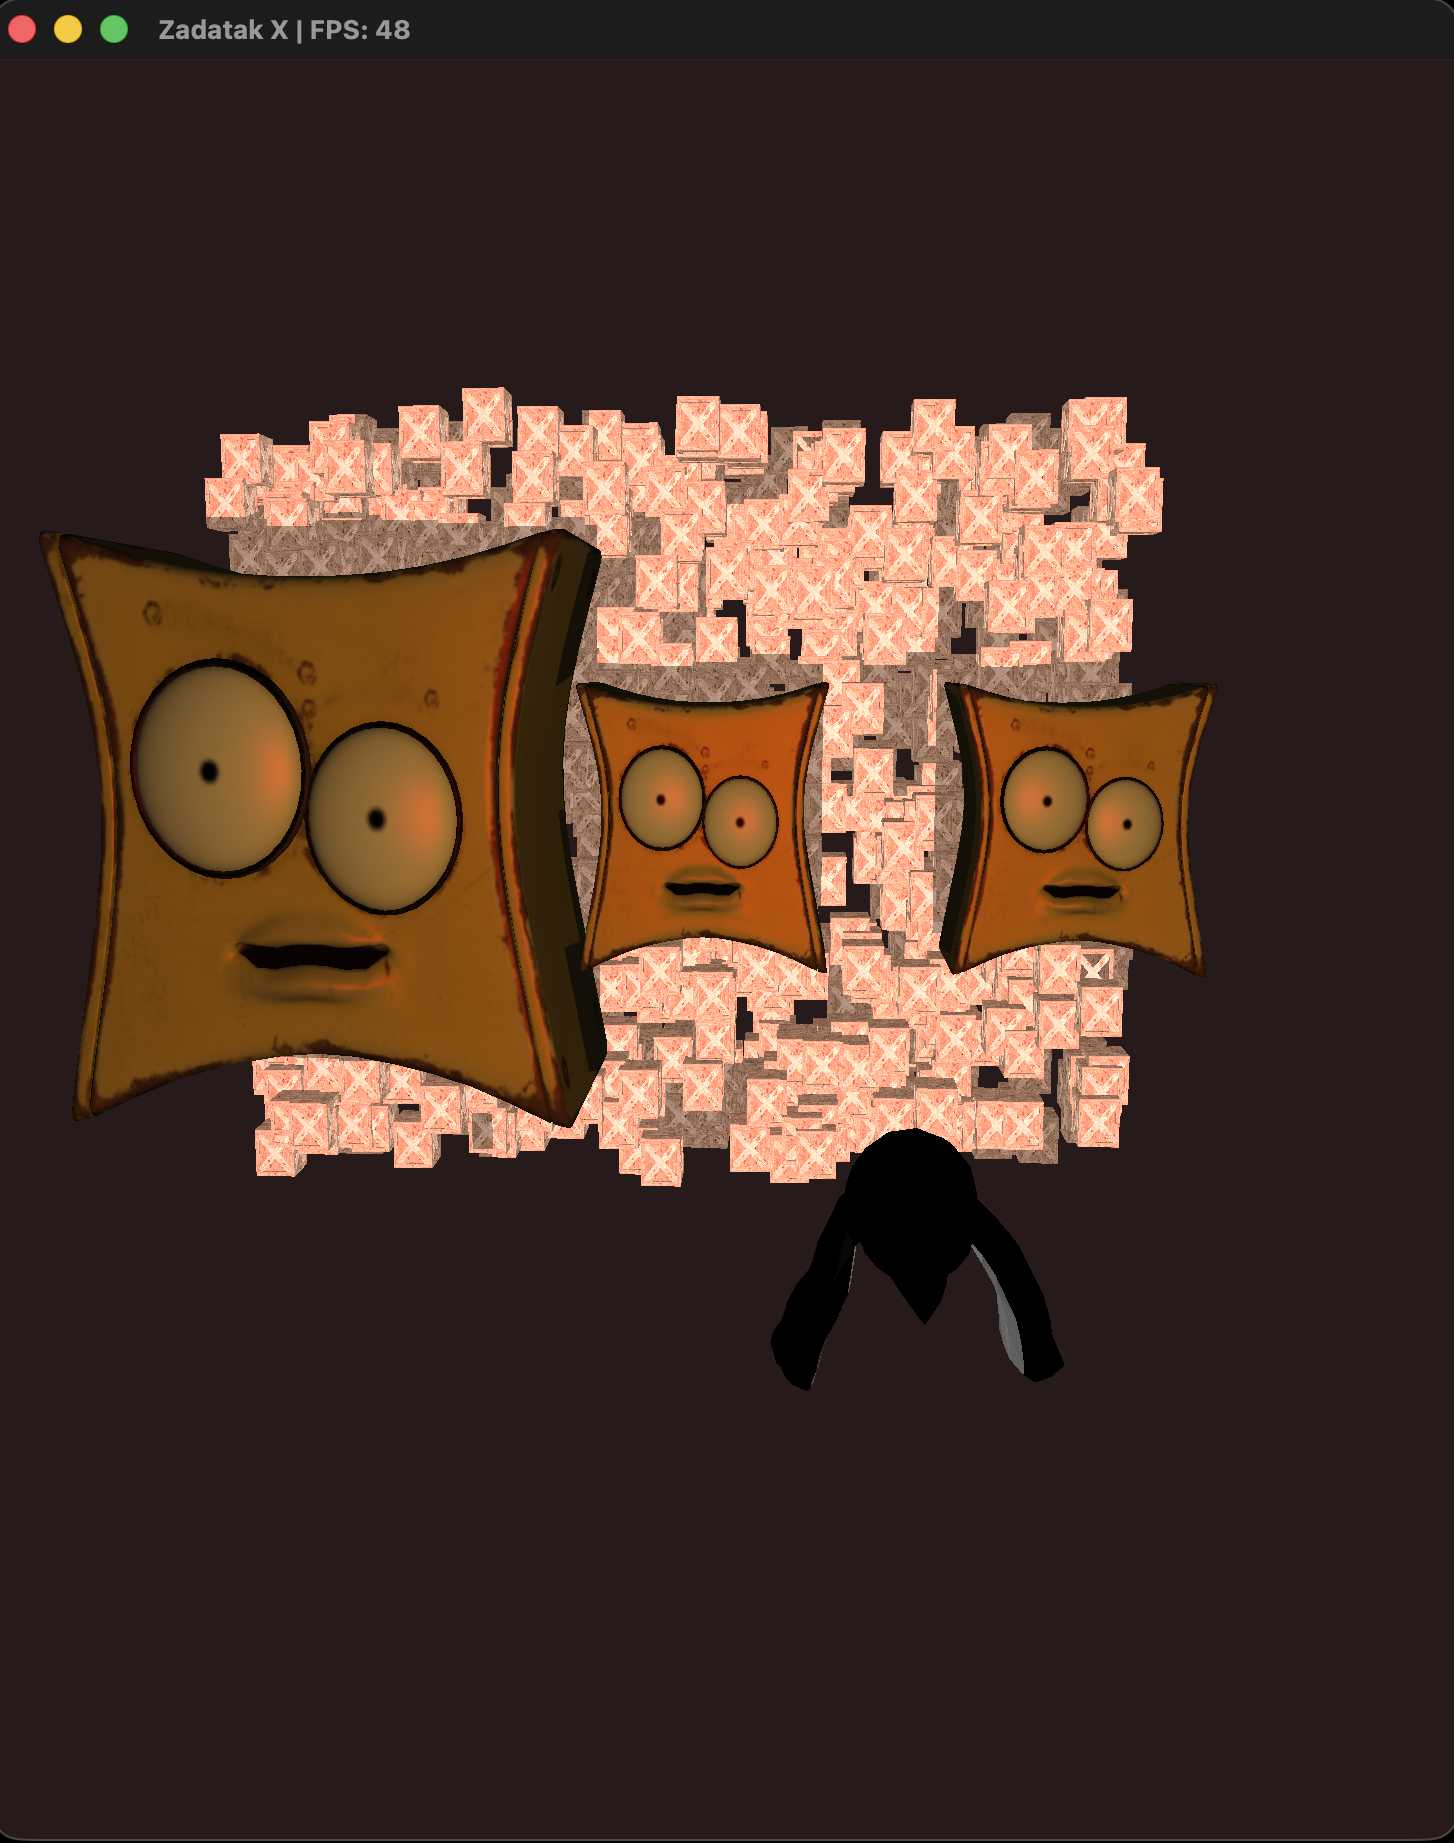
\includegraphics[width=0.5\textwidth]{figures/shadow_mapping.png}
    \caption{Example of the final shadow mapping pass. The objects in the scene accurately cast shadows onto each other based on the depth variance stored in the shadow framebuffer.}
    \label{fig:shadow_mapping}
\end{figure}












% --- 4. BIBLIOGRAPHY ---
\newpage
\printbibliography[heading=bibintoc, title={References}]

% --- 5. INDEX ---
\newpage
\printindex

\end{document}
